\documentclass[a4paper,12pt]{report}
\usepackage[T2A]{fontenc}
\usepackage[utf8]{inputenc}
\usepackage[english,russian]{babel}
\usepackage{graphicx}
\usepackage{wrapfig}
\usepackage{mathtext} 				% русские буквы в фомулах
\usepackage{amsmath,amsfonts,amssymb,amsthm,mathtools} % AMS
\usepackage{icomma} % "Умная" запятая: $0,2$ --- число, $0, 2$ --- перечисление
\usepackage{capt-of}
\usepackage{appendix}
\usepackage{multirow}
\usepackage{hyperref}
\usepackage{floatrow}
\usepackage[left=2cm,right=2cm,
    top=2cm,bottom=2cm,bindingoffset=0cm]{geometry}
\usepackage{multicol} % Несколько колонок
\usepackage{gensymb}
\title{Отчёт по лабораторной работе №6.11.2

Исследование фотопроводимости полупроводников}
\author{Плюскова Н.А. Б04-004 }
\date{\today}

\begin{document}

\maketitle

\section*{1. Аннотация}

В работе были исследованы собственная и примесная фотопроводимости. По полученной спектральной зависимости фототока была определена ширина запрещенной зоны и энергия ионизации примеси полупроводника.

\section*{2. Экспериментальная установка}

Схема экспериментальной установки изображена на рис. 1. 

\begin{center}
    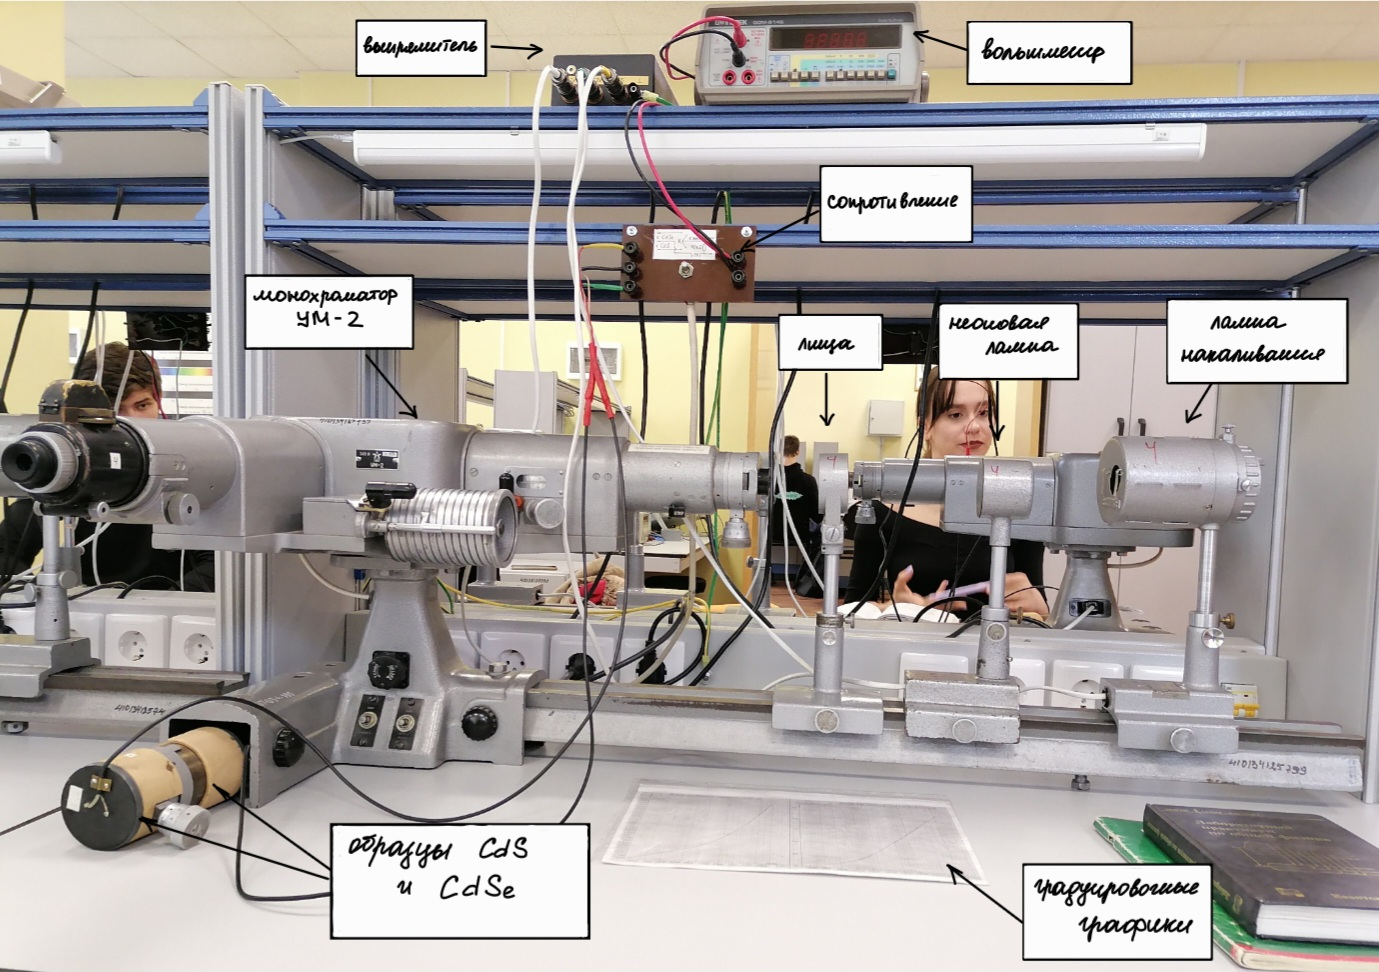
\includegraphics[width = \linewidth]{ustanovka.jpg}
    \captionof{figure}{ Схема экспериментальной установки}
\end{center}


Свет от источника И с помощью линзы Л фокусируется на вход щели монохроматора УМ-2. Эта щель находится в фокусе линзы Л1. 

\begin{center}
    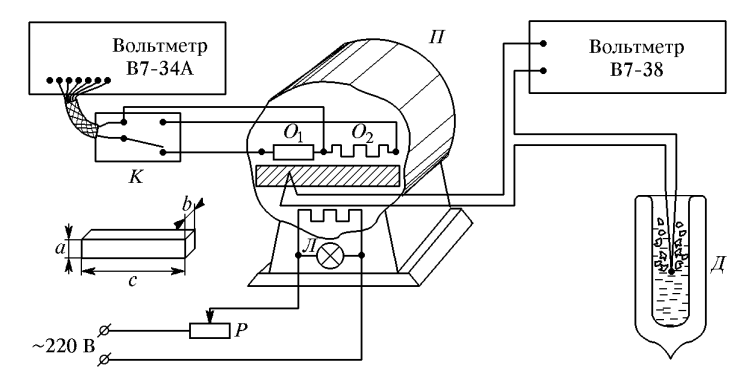
\includegraphics[width = \linewidth]{pic1.PNG}
    \captionof{figure}{ Схема установки для исследования спектральной зависимости фототока}
\end{center}


Параллельный пучок лучей, выходящий из линзы Л1, разлагается призмой П. Выходная щель находится в фокальной плоскости окулярной линзы 2 и вырезает из спектра нужную область. Прошедший сквозь выходную щель свет падает на ячейку с исследуемым образцом, обозначенную на рисунке буквой Я. Последовательно с образцом включены стабилизированный выпрямитель, служащий источником ЭДС. Вольтметр В7-34А служит для измерения тока, протекающего через образец.

Спектральное распределение потока фотонов на выходе монохроматора и градуировочная кривая монохроматора приведены на графиках, приложенных к работе.

\section*{3. Результаты эксперимента и обработка данных}
\subsection*{3.1 Градуировка монохроматора}
Проверив градуировку монохроматора с помощью желтой линии неоновой лампы, сдвинем градуировочный график вправо на 16 делений:


	\begin{figure}[H]
		\centering
		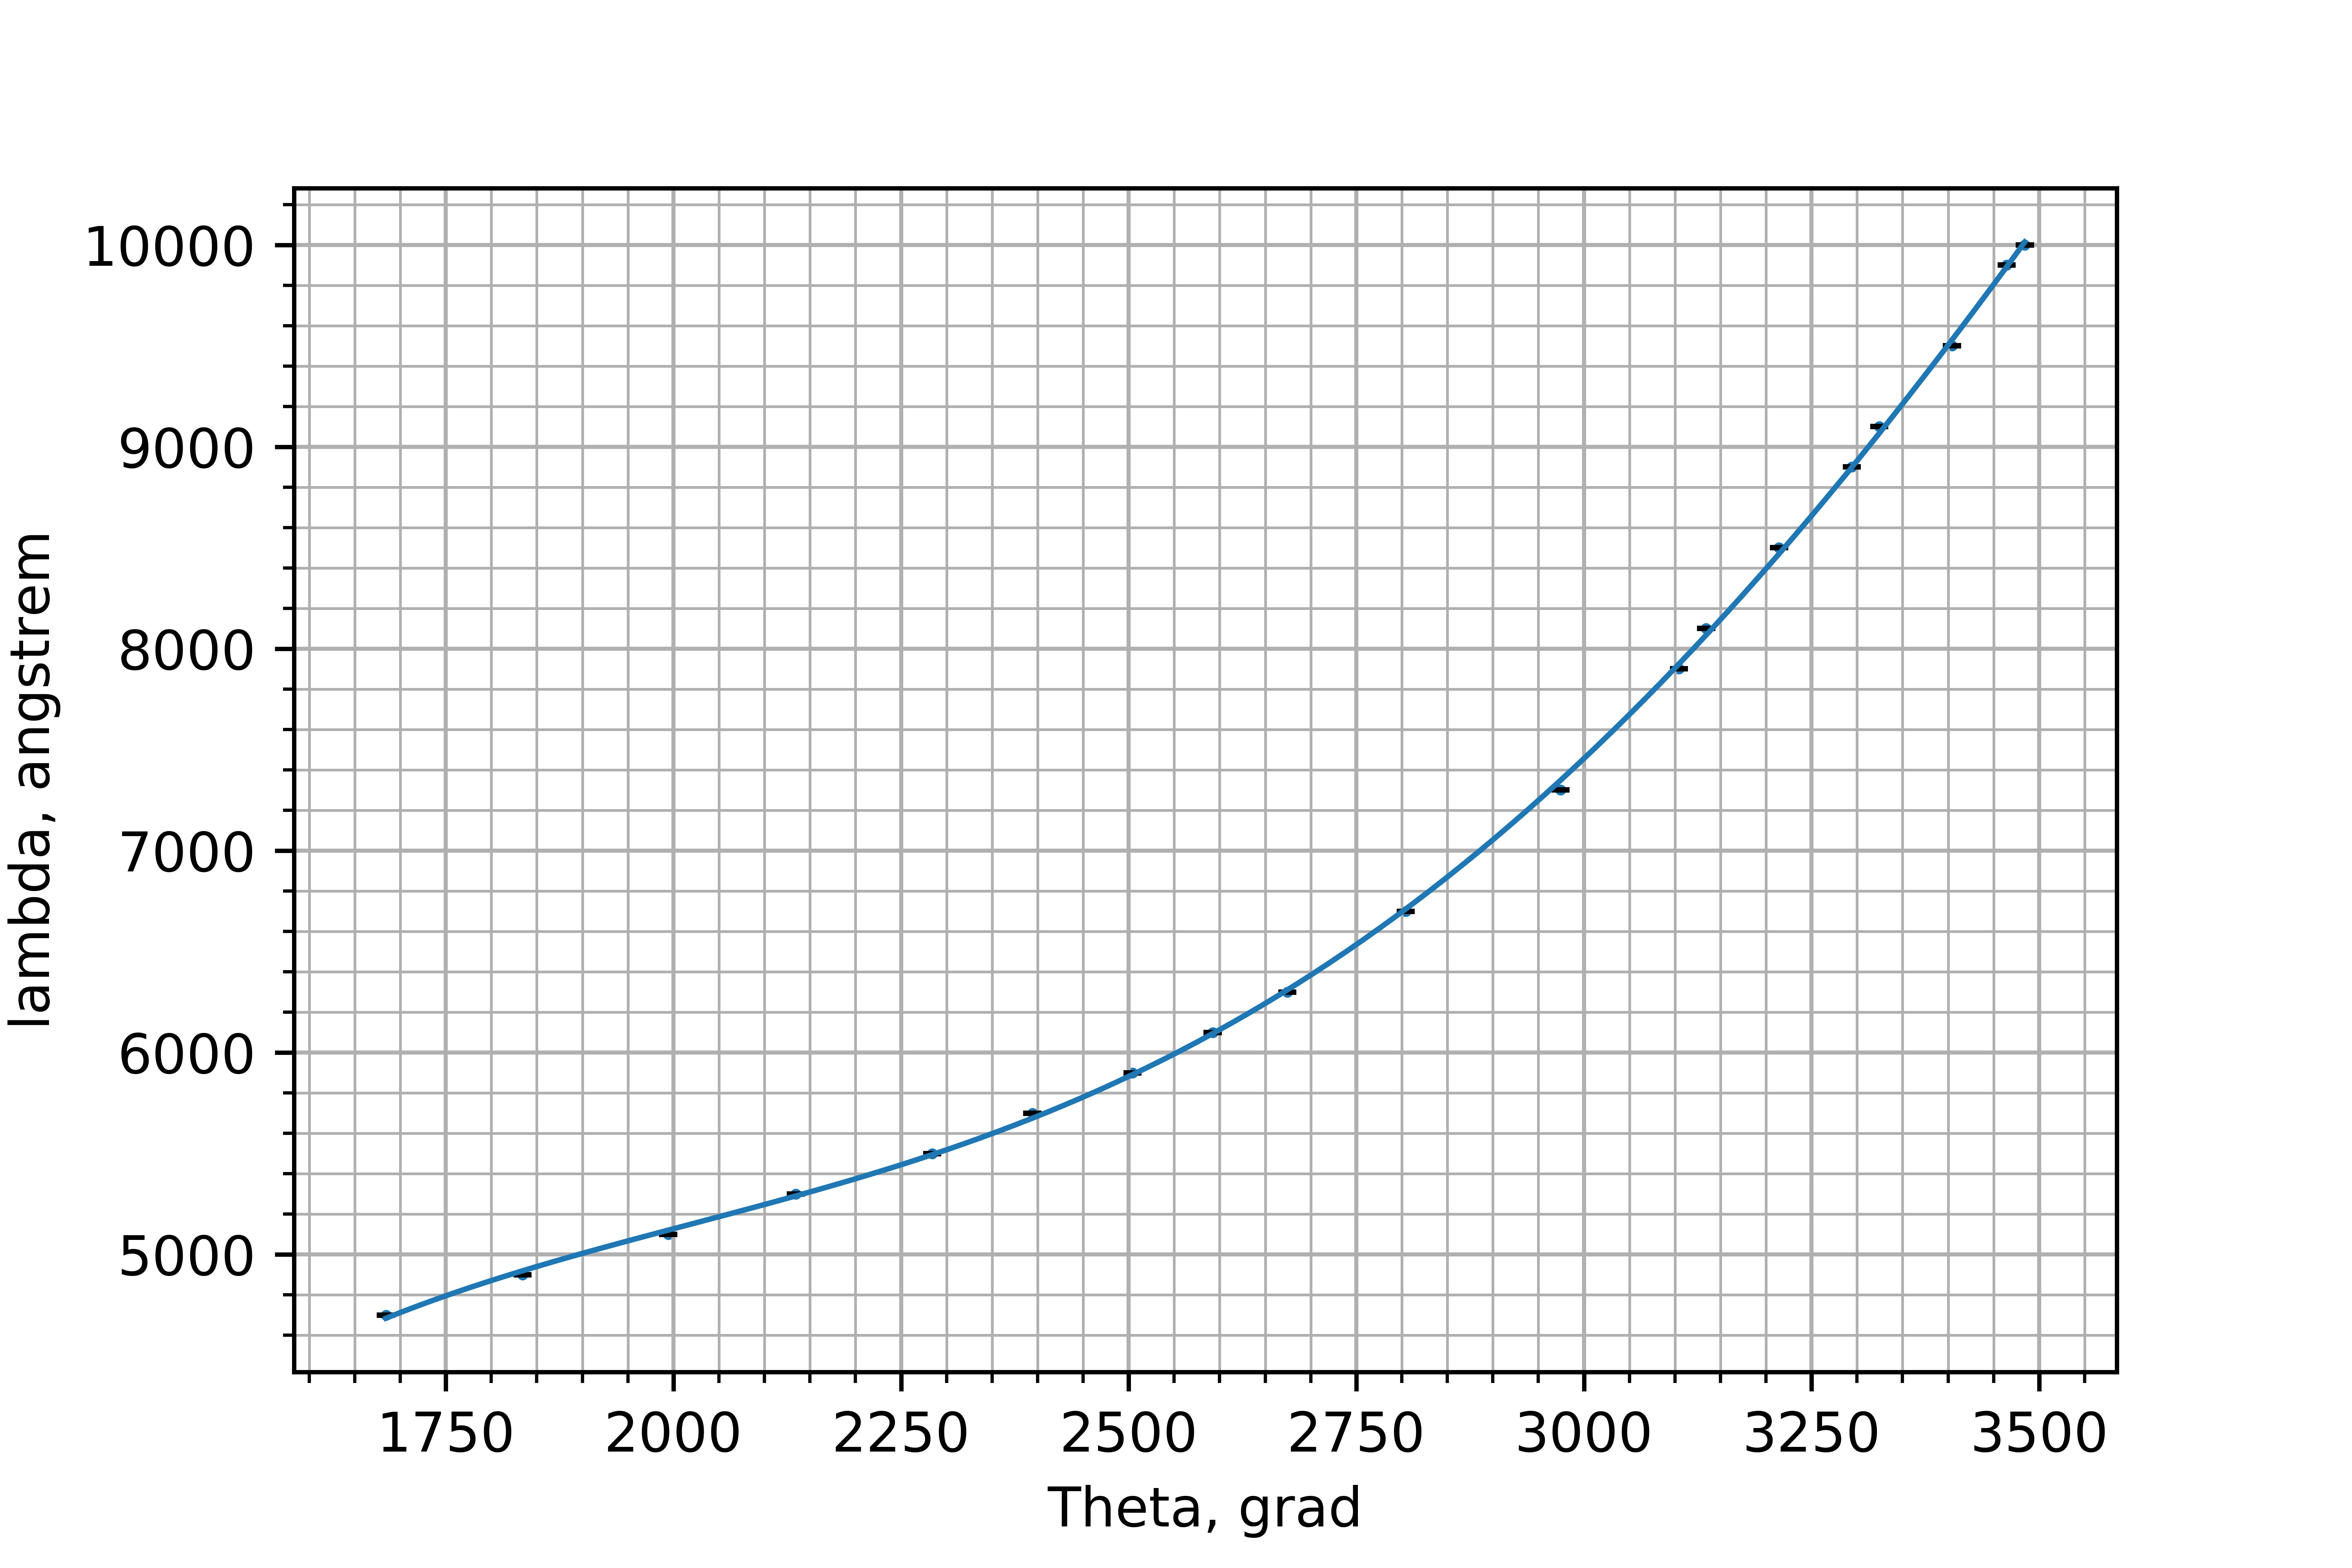
\includegraphics[width=0.7\linewidth]{grad.png}
		\caption{Градуировочная кривая $\lambda(\theta)$}
	\end{figure}
 
Получаем нелинейную градуировку, которую аппроксимируем полиномом 5 степени:
\begin{equation*}
    y = A + Bx + Cx^2 + Dx^3 + Ex^4
\end{equation*}
\begin{center}
$A = -17996; \ B = 35,6;\ C = -20,6 * 10^{-3};\ D = 51,8 * 10^{-7}; \ E = -4,39 * 10^{-10}$    
\end{center}
\subsection*{3.2 Нахождение ширины запрещенной зоны полупроводников}

Настроив монохроматор на измерение зависимости фототока от длины волны возбуждающего света, измерим темновой ток исследуемых образцов: CdS и CdSe.

\begin{equation*}
    I_{CdS_{\text{темн}}} = (5 \pm 0,3) \text{ мкА}
\end{equation*}

\begin{equation*}
    I_{CdS_{\text{темн}}} = (3\pm 0,3) \text{ мкА}
\end{equation*}

Снимем зависимость I($\lambda$), предварительно не забыв вычесть темновой ток из показаний вольтметра и пересчитав фототок к постоянному потоку фотонов:

\begin{table}[H]
\begin{center}
\begin{tabular}{|c|c|c|c|}
\hline
$\lambda, A^{o}$ & $\sigma_{\lambda}, A^{o}$ & $I$,нА & $\sigma_{I}$,нА \\ \hline
4856      & 2               & 2,5                         & 0,4                              \\ \hline
5163      & 2               & 5,8                         & 3,5                              \\ \hline
5310      & 2               & 10,5                        & 0,4                              \\ \hline
5354      & 2               & 11,8                        & 0,4                              \\ \hline
5389      & 2               & 13,0                        & 0,4                              \\ \hline
5473      & 2               & 16,3                        & 0,4                              \\ \hline
5519      & 3               & 17,5                        & 0,4                              \\ \hline
5599      & 3               & 20,3                        & 0,7                              \\ \hline
5685      & 3               & 23,8                        & 0,4                              \\ \hline
5780      & 3               & 27,3                        & 0,7                              \\ \hline
5882      & 3               & 31,5                        & 0,7                              \\ \hline
5993      & 3               & 35,5                        & 0,7                              \\ \hline
6113      & 3               & 40,0                        & 3,5                              \\ \hline
6243      & 4               & 45,0                        & 3,5                              \\ \hline
6384      & 4               & 50,0                        & 3,5                              \\ \hline
6513      & 4               & 55,0                        & 3,5                              \\ \hline
6696      & 4               & 60,0                        & 3,5                              \\ \hline
6869      & 5               & 62,5                        & 3,5                              \\ \hline
6884      & 5               & 61,5                        & 1,1                              \\ \hline
\end{tabular}
\hspace{1 cm}
\begin{tabular}{|c|c|c|c|}
\hline
$\lambda, A^{o}$ & $\sigma_{\lambda}, A^{o}$ & $I$,нА & $\sigma_{I}$,нА \\ \hline
6905      & 5               & 63,0                        & 1,8                              \\ \hline
6942      & 5               & 61,0                        & 1,4                              \\ \hline
7054      & 5               & 60,0                        & 3,5                              \\ \hline
7249      & 5               & 55,8                        & 1,8                              \\ \hline
7456      & 6               & 50,8                        & 1,4                              \\ \hline
7674      & 6               & 43,8                        & 1,8                              \\ \hline
7970      & 7               & 30,0                        & 3,5                              \\ \hline
8144      & 7               & 26,8                        & 1,8                              \\ \hline
8396      & 7               & 10,3                        & 0,7                              \\ \hline
8500      & 7               & 10,5                        & 0,7                              \\ \hline
8605      & 8               & 7,8                         & 0,7                              \\ \hline
8658      & 8               & 7,0                         & 0,7                              \\ \hline
8766      & 8               & 6,3                         & 0,7                              \\ \hline
9098      & 9               & 4,3                         & 0,4                              \\ \hline
9212      & 9               & 2,3                         & 0,4                              \\ \hline
9328      & 9               & 1,8                         & 0,7                              \\ \hline
9504      & 9               & 1,3                         & 0,4                              \\ \hline
9804      & 10              & 1,0                         & 0,4                              \\ \hline
\end{tabular}
\end{center}
\caption{Зависимость $I(\lambda)$ для CdS}
\end{table}

\begin{table}[H]
\begin{center}
\begin{tabular}{|c|c|c|c|}
\hline
$\lambda, A^{o}$ & $\sigma_{\lambda}, A^{o}$ & $I$,нА & $\sigma_{I}$,нА \\ \hline
5519      & 2               & 1,0                         & 0,4                              \\ \hline
5685      & 3               & 1,5                         & 0,4                              \\ \hline
5882      & 3               & 2,5                         & 0,4                              \\ \hline
6113      & 3               & 4,3                         & 0,4                              \\ \hline
6243      & 3               & 5,5                         & 0,4                              \\ \hline
6384      & 3               & 7,0                         & 0,4                              \\ \hline
6535      & 3               & 9,0                         & 0,7                              \\ \hline
6696      & 4               & 9,5                         & 0,7                              \\ \hline
6869      & 4               & 9,8                         & 1,4                              \\ \hline
6942      & 4               & 11,8                        & 0,7                              \\ \hline
6979      & 5               & 12,5                        & 0,7                              \\ \hline
7016      & 5               & 13,3                        & 0,7                              \\ \hline
7054      & 5               & 13,0                        & 0,4                              \\ \hline
7092      & 5               & 15,5                        & 0,7                              \\ \hline
7169      & 6               & 17,0                        & 0,7                              \\ \hline
7209      & 6               & 20,3                        & 0,4                              \\ \hline
7249      & 6               & 32,3                        & 0,7                              \\ \hline
\end{tabular}
\hspace{1cm}
\begin{tabular}{|c|c|c|c|}
\hline
$\lambda, A^{o}$ & $\sigma_{\lambda}, A^{o}$ & $I$,нА & $\sigma_{I}$,нА \\ \hline
7330      & 6               & 70,0                        & 1,8                              \\ \hline
7372      & 7               & 100,8                       & 1,8                              \\ \hline
7456      & 7               & 170,5                       & 1,4                              \\ \hline
7499      & 7               & 190,5                       & 1,8                              \\ \hline
7542      & 8               & 194,5                       & 3,5                              \\ \hline
7586      & 8               & 192,0                       & 3,5                              \\ \hline
7630      & 9               & 187,3                       & 1,8                              \\ \hline
7674      & 9               & 184,5                       & 3,5                              \\ \hline
7719      & 10              & 181,3                       & 1,8                              \\ \hline
7765      & 10              & 175,3                       & 1,8                              \\ \hline
7904      & 10              & 159,5                       & 1,8                              \\ \hline
7904      & 10              & 170,3                       & 1,8                              \\ \hline
8144      & 11              & 136,0                       & 1,8                              \\ \hline
8396      & 11              & 102,0                       & 3,5                              \\ \hline
8658      & 11              & 80,5                        & 1,8                              \\ \hline
8930      & 12              & 64,0                        & 0,7                              \\ \hline
9212      & 13              & 50,5                        & 0,7                              \\ \hline
\end{tabular}
\caption{Зависимость $I(\lambda)$ для CdSe}
\end{center}
\end{table}

Построим соответствующие графики:

	\begin{figure}[H]
		\centering
		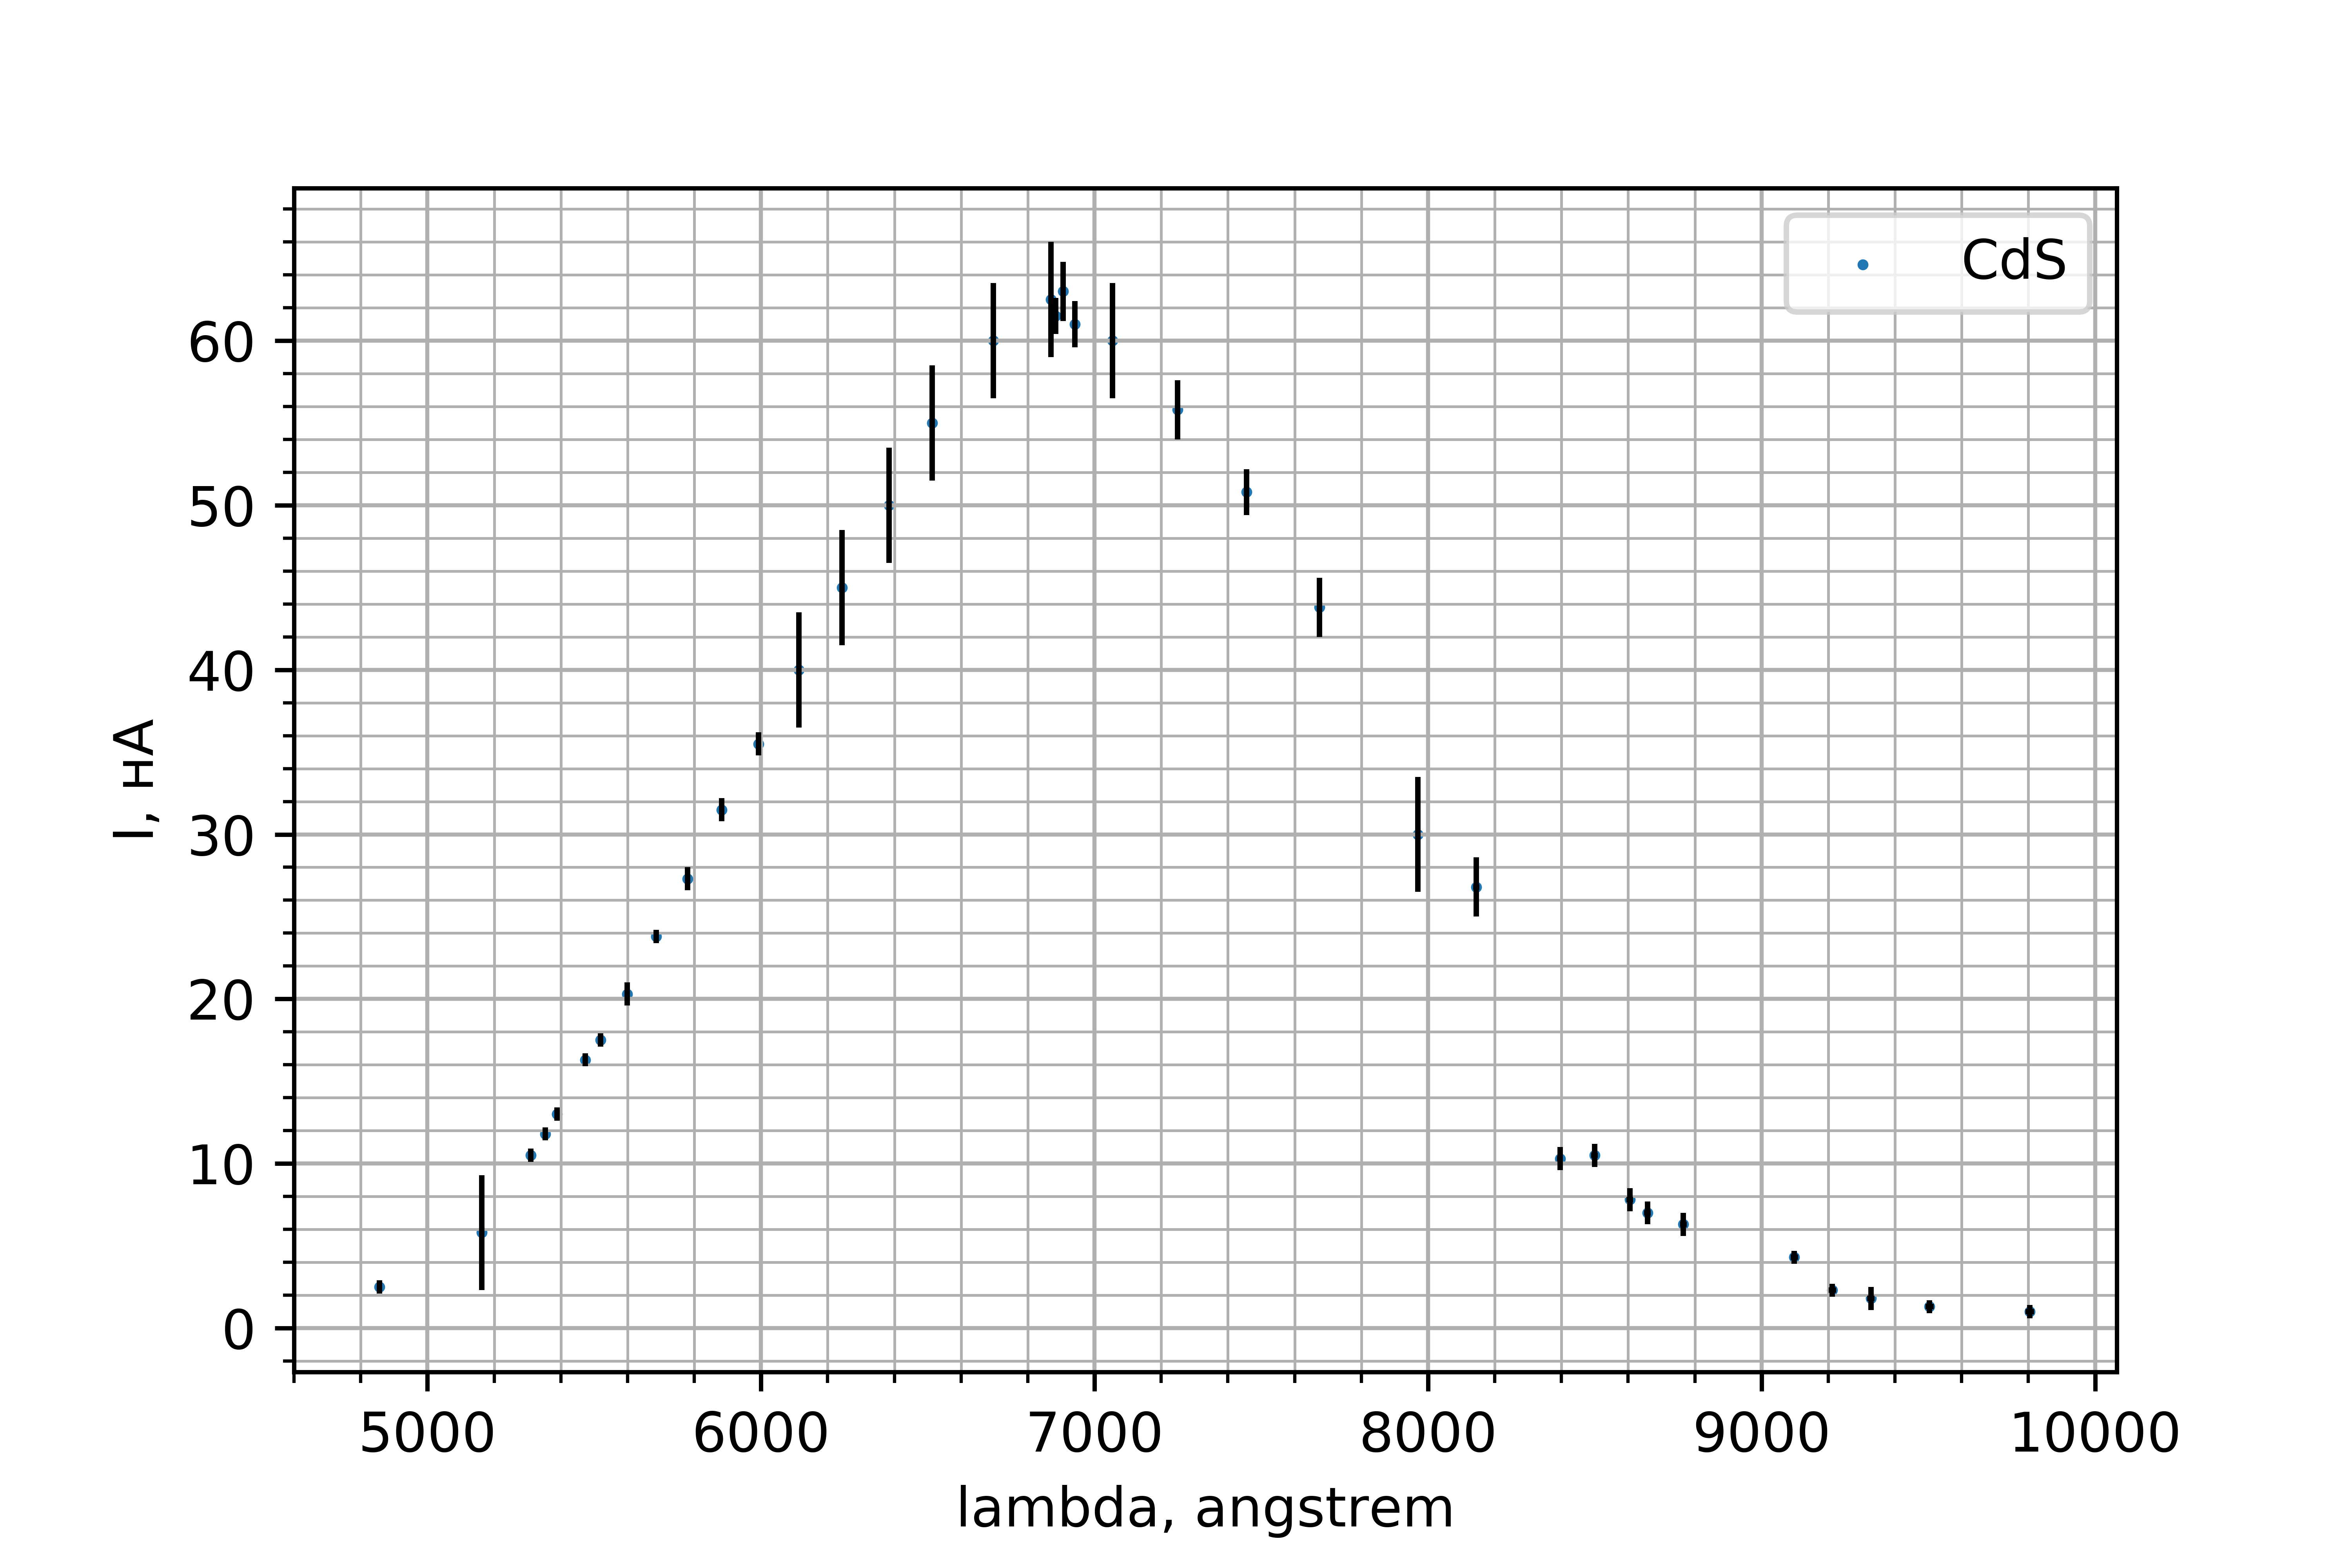
\includegraphics[width=0.7\linewidth]{CdS.png}
		\caption{Зависимость $I(\lambda)$ для CdS}
	\end{figure}

 
	\begin{figure}[H]
		\centering
		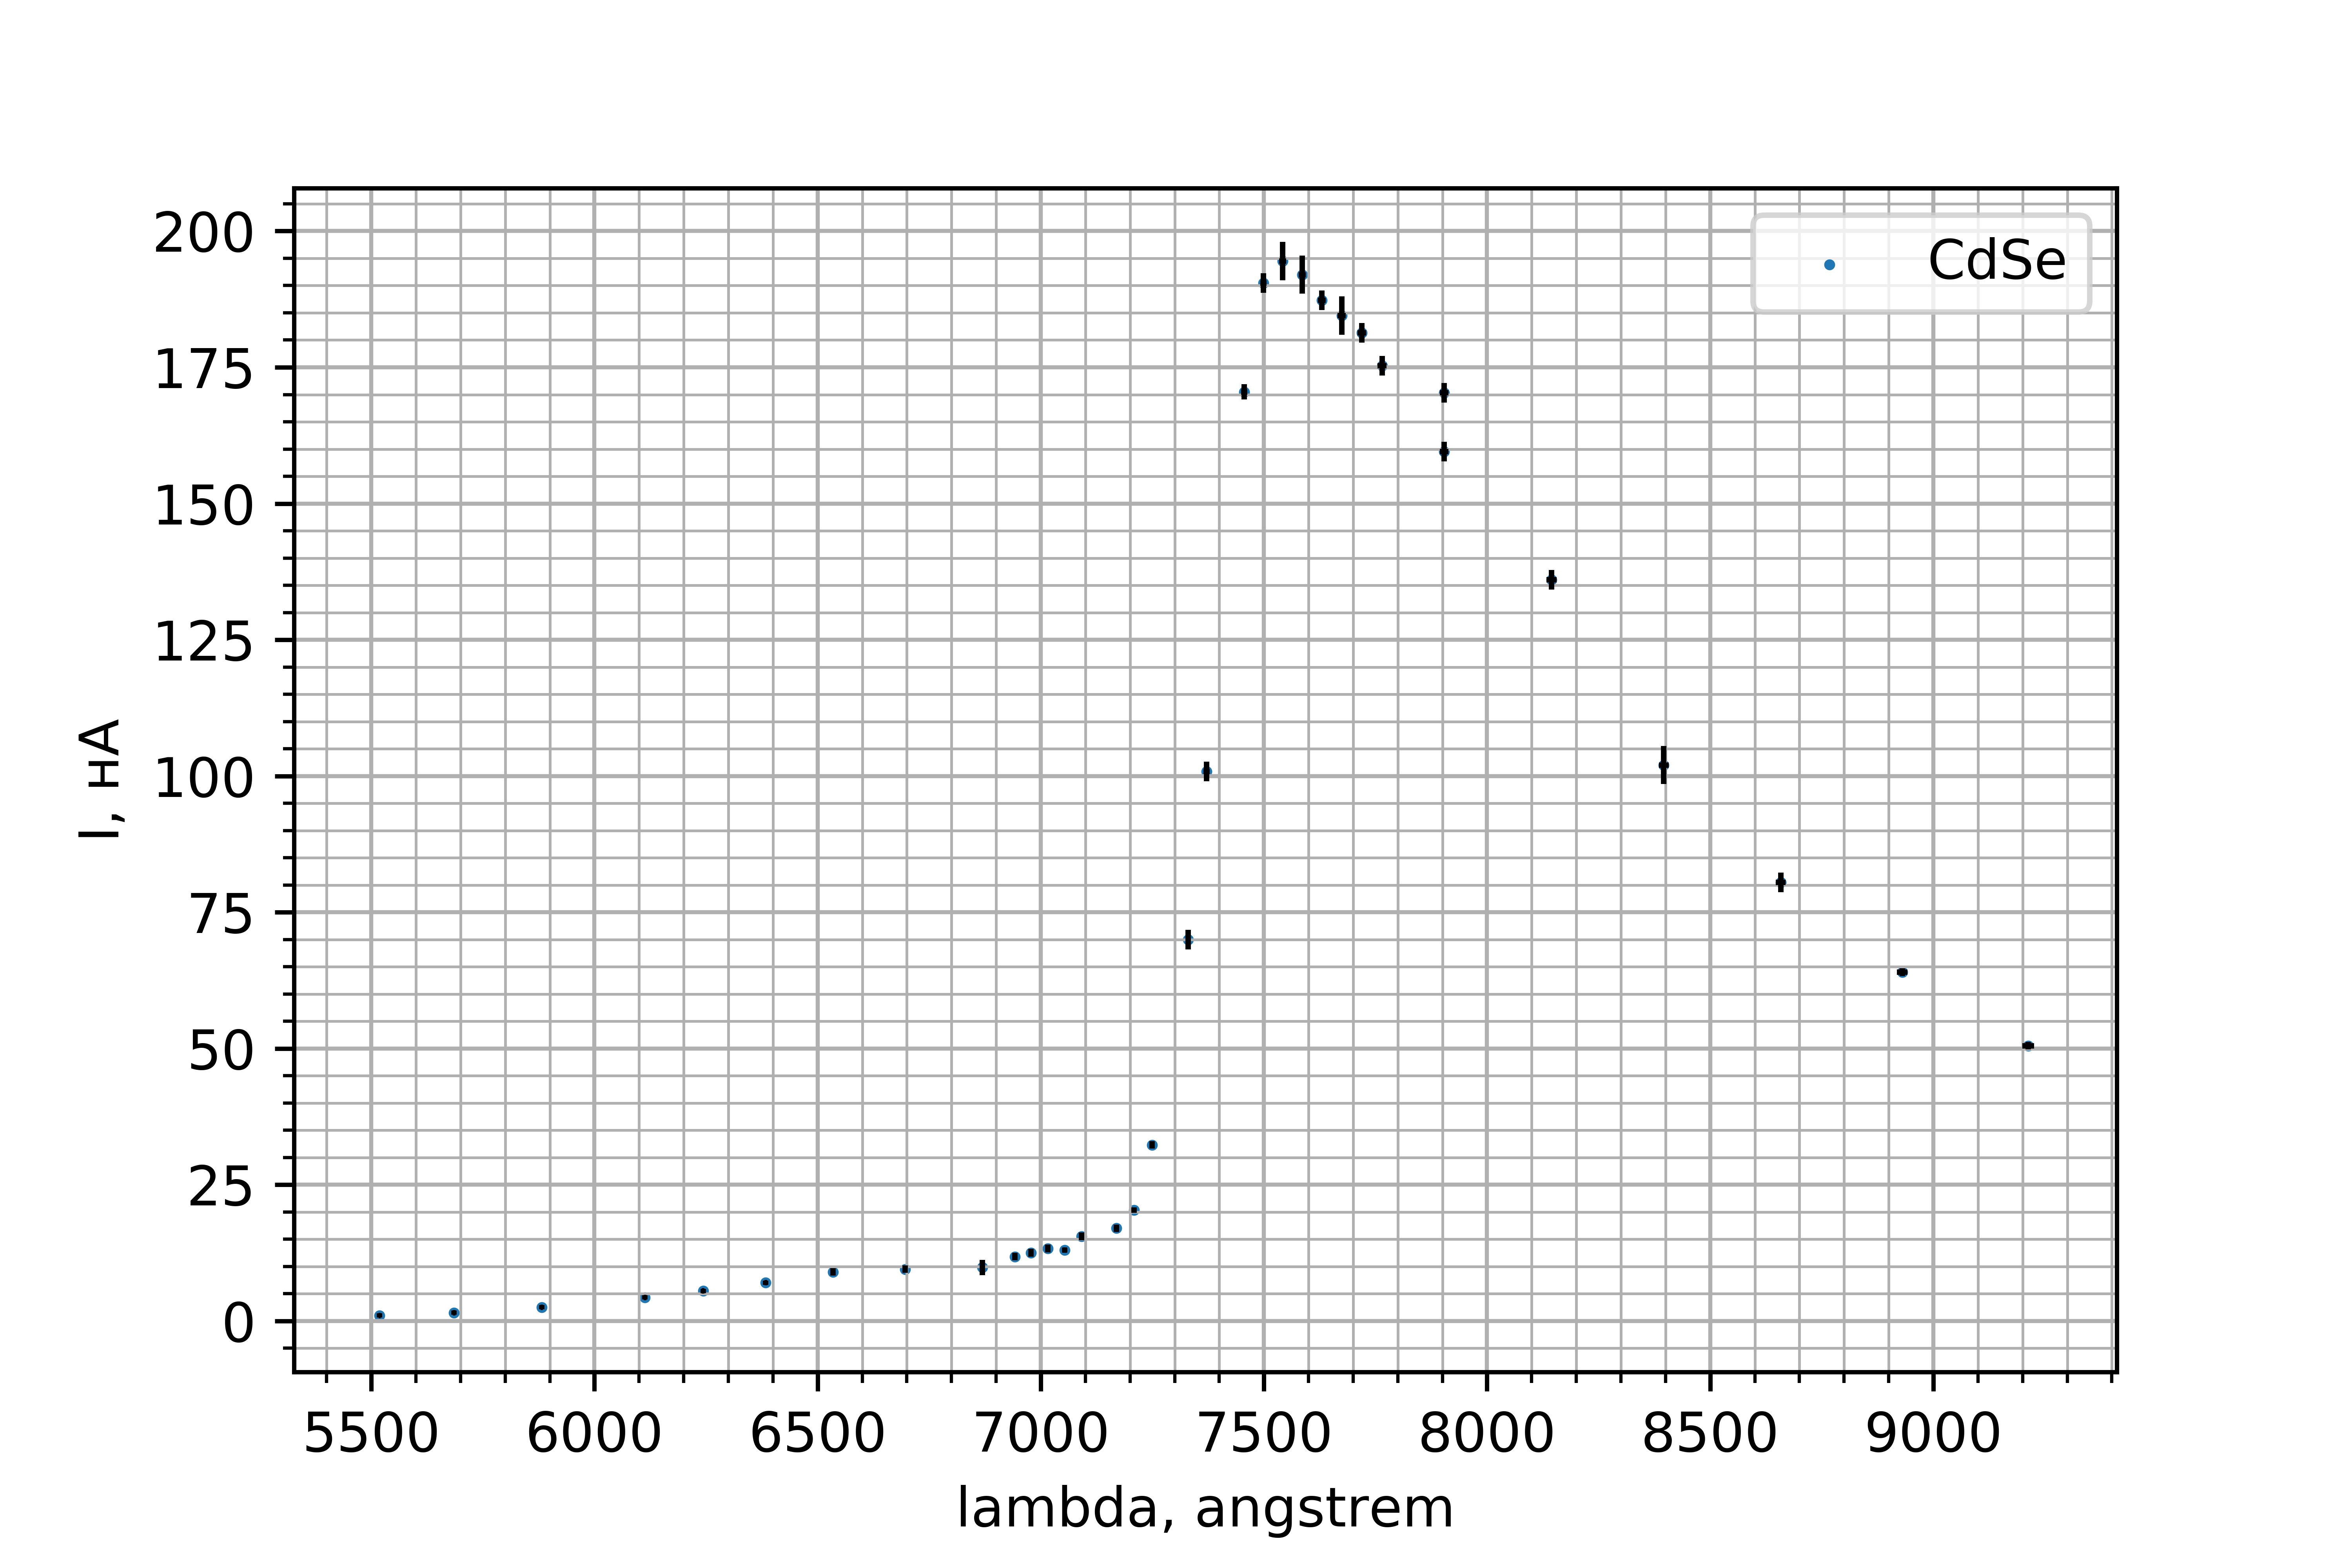
\includegraphics[width=0.7\linewidth]{CdSe.png}
		\caption{Зависимость $I(\lambda)$ для CdSe}
	\end{figure}

 Из графика найдем красные границы фотоэффекта:
 \begin{equation*}
     \lambda_{CdS_{\text{кр}}} = (6010\pm 13) A^{o} 
 \end{equation*}

  \begin{equation*}
     \lambda_{CdSe_{\text{кр}}} = (7414\pm 13) A^{o} 
 \end{equation*}

По найденным длинам волн оценим ширину запрещенной зоны полупроводников:

  \begin{equation*}
     \Delta_{CdS} = (2,04 \pm 0,01) \text{ эВ} 
 \end{equation*}

  \begin{equation*}
     \Delta_{CdSe} = (1,67 \pm 0,01) \text{ эВ} 
 \end{equation*}

 Отметим, что значение $\Delta_{CdSe} = (1,67 \pm 0,01) \text{ эВ}$ в пределах $2\%$ совпадает с теоретическим ($\Delta_{CdSe_{\text{теор}}} = 1,7 $ эВ)

\section*{4. Вывод}

В работе была исследована собственная фотопроводимость полупроводников и построены графики зависимости фототока для образцов $CdS$ и $CdSe$; по графикам были определены ширина запрещенной зоны. 

Для образцов не наблюдаются примесные пики фотопроводимости. Возможно, для $CdSe$ они находятся в области $\lambda \sim 7300 A^{o}$, которая была плохо промерена. Также данную картину можно наблюдать, если примесей в полупроводнике мало.

Также следует отметить, что найденные нами погрешности не совпадают с реальными вследствие следующих причин:
\begin{itemize}
    \item Мы не учитываем погрешность данного нам градуировочного графика, а также погрешность глаза.
    \item Возможно, нельзя по одной линии из всего спектра судить, в какую сторону нужно сдвигать график. По моему мнению, зависимость более сложная и индивидуальна для каждой установки.
    \item Желтая линия спектра неона могла быть определена неверно, т.к. засветка от лампы накаливания и ламп, освещающих кабинет, в котором происходили измерения, вносила дополнительные линии, которые не имели отношения к спектру неона.
\end{itemize}

\end{document}
